\documentclass[a4paper, 12pt]{article}

% \usepackage[portuges]{babel}
\usepackage[utf8]{inputenc}
\usepackage{subfig}
\usepackage[colorinlistoftodos]{todonotes}

\usepackage[english]{babel}
\usepackage{indentfirst,setspace,subcaption}
\usepackage{amsmath,amssymb,graphicx,xcolor,url}
\usepackage{fancyhdr,tocbasic,titlesec,minted,listings}
\usepackage[a4paper,margin=24mm]{geometry}
\usepackage[skip=10pt plus1pt, indent=20pt]{parskip}
\usepackage[colorlinks=true,allcolors=blue,urlcolor=magenta]{hyperref}

\usepackage{indentfirst}
\usepackage{verbatim}
\usepackage{textcomp}
\usepackage{gensymb}

\usepackage{relsize}

\usepackage{lipsum}% http://ctan.org/pkg/lipsum
\usepackage{xcolor}% http://ctan.org/pkg/xcolor
\usepackage{xparse}% http://ctan.org/pkg/xparse
\NewDocumentCommand{\myrule}{O{1pt} O{2pt} O{black}}{%
  \par\nobreak % don't break a page here
  \kern\the\prevdepth % don't take into account the depth of the preceding line
  \kern#2 % space before the rule
  {\color{#3}\hrule height #1 width\hsize} % the rule
  \kern#2 % space after the rule
  \nointerlineskip % no additional space after the rule
}
\usepackage[section]{placeins}

\usepackage{booktabs}
\usepackage{colortbl}%
   \newcommand{\myrowcolour}{\rowcolor[gray]{0.925}}
   

\pagestyle{fancy}
\setlength{\headheight}{15pt}
\fancyhf{}
\fancyhead[R]{\nouppercase\rightmark\hfill~Exercise I Report}
\fancyfoot[C]{\hfill\thepage\hfill}

\DeclareTOCStyleEntry[
  indent=12pt,
  level=1
]{largetocline}{section}

\setlength {\marginparwidth }{2cm} 
\begin{document}
\begin{titlepage}
\begin{center}
\textbf{\LARGE Vietnam National University,}\\[0.5cm] 
\textbf{\LARGE Ho Chi Minh City}\\[0.5cm] 
\vspace{20pt}
\textbf{\large UNIVERSITY OF SCIENCE}\\[0.2cm]
\textbf{\large FACULTY OF INFORMATION TECHNOLOGY}\\[0.2cm]
\vspace{20pt}

\includegraphics[width=0.5\textwidth,keepaspectratio]{images/logo.png}

\par
\vspace{20pt}
\textbf{\Large CSC10004 - Data Structure And Algorithms}\\
\vspace{15pt}
\myrule[1pt][7pt]
\textbf{\LARGE EXERCISE I REPORT}\\
\vspace{15pt}
\textbf{\large Implementing Stack and Queue from scratch}\\
\vspace{10pt}
\myrule[1pt][7pt]
\vspace{25pt}
\textbf{\large Student Name \hspace{20pt} Student ID}\\
Bui Minh Duy \hspace{45pt} 23127040 \\ 

\vspace{45pt}
\textbf {\large Lecturer in charge:}\\[0.2cm]
\Large {Bui Duy Dang}\\[0.1cm]
\Large {Nguyen Thanh Tinh}\\[0.1cm]
\end{center}

\par
\vfill
\begin{center}
\text{16/06/2024}\\
\end{center}

\end{titlepage}

\tableofcontents\thispagestyle{empty}

\pagebreak
\section{Experiment Details}
\thispagestyle{empty}
\subsection{Stack Array}
\subsubsection*{Push Operation}
\begin{figure}[H]
	\centering
        \subfloat[\centering Normal case]{\includegraphics[width=6cm]{images/stack/array/push_normal.png}}
        \qquad
        \subfloat[\centering Full case]{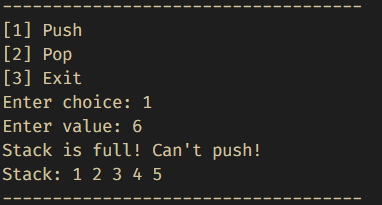
\includegraphics[width=6cm]{images/stack/array/push_full.png}}
	\vfill
	\caption{Push elements in Stack Array of size 5}\label{fig:stack_arr_push}
\end{figure}
\subsubsection*{Pop Operation}
\begin{figure}[H]
	\centering
        \subfloat[\centering Normal case]{\includegraphics[width=6cm]{images/stack/array/pop_normal.png}}
        \qquad
        \subfloat[\centering Empty case]{\includegraphics[width=6cm]{images/stack/array/pop_empty.png}}
        \vfill
	\caption{Pop elements in Stack Array of size 5}\label{fig:stack_arr_pop}
\end{figure}

\pagebreak
\subsection{Stack Linked List}
\subsubsection*{Push Operation}
\begin{figure}[H]
	\centering
        \subfloat[\centering Normal Case] {\includegraphics[width=0.7\textwidth]{images/stack/linked_list/push_normal.png}}
	\caption{Push elements in Stack Linked List}\label{fig:stack_ll_push}
\end{figure}
\subsubsection*{Pop Operation}
\begin{figure}[H]
	\centering
        \subfloat[\centering Normal case]{\includegraphics[width=6cm]{images/stack/linked_list/pop_normal.png}}
        \qquad
        \subfloat[\centering Empty case]{\includegraphics[width=6cm]{images/stack/linked_list/pop_empty.png}}
        \vfill
	\caption{Pop elements in Stack Linked List}\label{fig:stack_ll_pop}
\end{figure}
\thispagestyle{empty}
\pagebreak
\subsection{Queue Array}
\subsubsection*{Enqueue Operation}
\begin{figure}[H]
	\centering
        \subfloat[\centering Normal case]{\includegraphics[width=6cm]{images/queue/array/enqueue_normal.png}}
        \qquad
        \subfloat[\centering Full case]{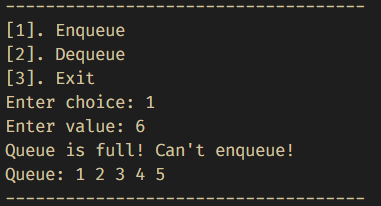
\includegraphics[width=6cm]{images/queue/array/enqueue_full.png}}
        \vfill
	\caption{Enqueue elements in Queue Array of size 5}\label{fig:queue_arr_enqueue}
\end{figure}
\subsubsection*{Dequeue Operation}
\begin{figure}[H]
	\centering
        \subfloat[\centering Normal case]{\includegraphics[width=6cm]{images/queue/array/dequeue_normal.png}}
	\qquad
        \subfloat[\centering Empty case]{\includegraphics[width=6cm]{images/queue/array/dequeue_empty.png}}
	\caption{Dequeue elements in Queue Array of size 5}\label{fig:queue_arr_dequeue}
\end{figure}

\pagebreak
\subsection{Queue Linked List}
\subsubsection*{Enqueue Operation}
\begin{figure}[H]
        \centering
        \subfloat[\centering Normal case]{\includegraphics[width=0.7\textwidth]{images/queue/linked_list/enqueue_normal.png}}
	\caption{Enqueue elements in Queue Linked List}\label{fig:queue_ll_enqueue}
\end{figure}
\subsubsection*{Dequeue Operation}
\begin{figure}[H]
	\centering
        \subfloat[\centering Normal case]{\includegraphics[width=6cm]{images/queue/linked_list/dequeue_normal.png}}
	\qquad
        \subfloat[\centering Empty case]{\includegraphics[width=6cm]{images/queue/linked_list/dequeue_empty.png}}
	\caption{Dequeue elements in Queue Linked List}\label{fig:queue_ll_dequeue}
\end{figure}

\pagebreak
\section{Recursive versions}
\thispagestyle{empty}
\subsection{Stack}
\subsubsection*{Recursive Stack Array}
\begin{itemize}
	\item \textbf{Theoretical Time Complexity:} Both implementations have the same theoretical time complexity of O(n) for \verb|copy| operations.
	\item \textbf{Actual execution time:} 
\end{itemize}
\begin{figure}[H]
	    \centering
	    \includegraphics[width=0.8\textwidth]{images/recursive_stack/array/copy_time.png}
	    \caption{Comparison between Loop version and Recursive version}\label{fig:rs_arr_copy_time}
        \end{figure}
\subsubsection*{Recursive Stack Linked List}
\begin{itemize}
	\item \textbf{Theoretical Time Complexity:} Both implementations have the same theoretical time complexity of O(n) for \verb|copy| and \verb|release| operations.
	\item \textbf{Actual execution time:}
\end{itemize}
\begin{figure}[H]
        \centering
        \includegraphics[width=0.8\textwidth]
         {images/recursive_stack/linked_list/copy_time.png}
        \caption{Comparison between Loop version and Recursive version}\label{fig:rs_ll_copy_time}
        \hfill
        \vfill
        \centering
        \includegraphics[width=0.8\textwidth]
        {images/recursive_stack/linked_list/release_time.png}
        \caption{Comparison between Loop version and Recursive version}\label{fig:rs_ll_release_time}
\end{figure}
\thispagestyle{empty}
\subsection{Queue}
\subsubsection*{Recursive Queue Array}
\begin{itemize}
	\item \textbf{Theoretical Time Complexity:} Both implementations have the same theoretical time complexity of O(n) for \verb|copy| operations.
	\item \textbf{Actual execution time:}
\end{itemize}
\begin{figure}[H]
	\centering
	\includegraphics[width=0.8\textwidth]{images/recursive_queue/array/copy_time.png}
	\caption{Comparison between Loop version and Recursive version}\label{fig:rq_arr_copy_time}
\end{figure}

\subsubsection*{Recursive Queue Linked List}
\begin{itemize}
	\item \textbf{Theoretical Time Complexity:} Both implementations have the same theoretical time complexity of O(n) for \verb|copy| and \verb|release| operations.
	\item \textbf{Actual execution time:}
\end{itemize}
\begin{figure}[!ht]
	\centering
        \includegraphics[width=0.8\textwidth]{images/recursive_queue/linked_list/copy_time.png}
        \caption{Comparison between Loop version and Recursive version}\label{fig:rq_ll_copy_time}
	\hfill
        \vfill
        \centering
        \includegraphics[width=0.8\textwidth]{images/recursive_queue/linked_list/release_time.png}
        \caption{Comparison between Loop version and Recursive version}\label{fig:rq_ll_release_time}
\end{figure}

\subsection{Conclusion}
\begin{itemize}
    \item Though Loop version and Recursive Version have the same theoretical time complexity of O(n), the actual execution time shows that Loop version is faster in all cases.
    \item When working with large data sets, the Loop version still executes as normal, but the Recursive version might encounter Stack Overflow.
\end{itemize}

\pagebreak
\section{Self-evaluation}
\begin{center}
  \renewcommand{\arraystretch}{1.5}
  \begin{tabular}{|l|p{\dimexpr0.6\linewidth-2\tabcolsep}|c|}
    \hline
    \textbf{No.} & \textbf{Details}            & \textbf{Score} \\ \hline
    1            & Stack Array                 & 100\%          \\ \hline
    2            & Stack Linked List           & 100\%          \\ \hline
    3            & Queue Array                 & 100\%          \\ \hline
    4            & Queue Linked List           & 100\%          \\ \hline
    5            & Recursive versions          & 100\%          \\ \hline
    6            & Report                      & 100\%          \\ \hline
                 & \textbf{Overall}            & \textbf{100\%} \\ \hline
  \end{tabular}
\end{center}

\section{Exercise Feedback}
\subsection{What I learned}
\begin{flushleft}
\begin{itemize}
    \item Better understanding about the internal processing of stack and queue.
    \item How to use function templates in C++. 
\end{itemize}
\end{flushleft}
\subsection{What was difficult}
\begin{flushleft}
\begin{itemize}
    \item The approach of using recursion is quite challenging, it took a significant amount of time and effort to complete the set-up.
\end{itemize}
\end{flushleft}

\end{document}

\end{document}